\documentclass[../main.tex]{subfiles}
\begin{document}

\theoremstyle{definition}

\chapter{Gauss Elimination}
\label{cha9:cha9}
\begin{center}
\Large{\textbf{CHAPTER OBJECTIVES}}
\end{center}

The primary objective of this chapter is to describe the Gauss elimination algorithm for solving linear algebraic equations. Specific objectives and topics covered are
\begin{itemize}
\item Knowing how to solve small sets of linear equations with the graphical method and Cramer's rule.
\item Understanding how to implement forward elimination and back substitution as in Gauss elimination.
\item Understanding how to count flops to evaluate the efficiency of an algorithm.
\item Understanding the concepts of singularity and ill-condition.
\item Understanding how partial pivoting is implemented and how it differs from complete pivoting.
\item Knowing how to compute the determinant as part of the Gauss elimination algorithm with partial pivoting.
\item Recognizing how the banded structure of a tridiagonal system can be exploited to obtain extremely efficient solutions.
\end{itemize}
\bigskip

At the end of Chap. 8, we stated that MATLAB provides two simple and direct methods for solving systems of linear algebraic equations: left division,

\begin{lstlisting}[numbers=none,frame=none]
    >> x = A\b
\end{lstlisting}

and matrix inversion,

\begin{lstlisting}[numbers=none,frame=none]
    >> x = inv(A)*b
\end{lstlisting}

Chapters 9 and 10 provide background on how such solutions are obtained. This material is included to provide insight into how MATLAB operates. In addition, it is intended to show how you can build your own solution algorithms in computational environments that do not have MATLAB's built-in capabilities.

The technique described in this chapter is called Gauss elimination because it involves combining equations to eliminate unknowns. Although it is one of the earliest methods for solving simultaneous equations, it remains among the most important algorithms in use today and is the basis for linear equation solving on many popular software packages including MATLAB.

\newpage
\section{SOLVING SMALL NUMBERS OF EQUATIONS}
\label{sec:sec_9_1}

Before proceeding to Gauss elimination, we will describe several methods that are appropriate for solving small $(n \leq 3)$ sets of simultaneous equations and that do not require a computer. These are the graphical method, Cramer's rule, and the elimination of unknowns.

\subsection{The Graphical Method}

A graphical solution is obtainable for two linear equations by plotting them on Cartesian coordinates with one axis corresponding to $x_{1}$ and the other to $x_{2}$. Because the equations are linear, each equation will plot as a straight line. For example, suppose that we have the following equations:
$$
\begin{aligned}
3 x_{1}+2 x_{2} &=18 \\
-x_{1}+2 x_{2} &=2
\end{aligned}
$$
If we assume that $x_{1}$ is the abscissa, we can solve each of these equations for $x_{2}$ :
$$
\begin{aligned}
&x_{2}=-\frac{3}{2} x_{1}+9 \\
&x_{2}=\frac{1}{2} x_{1}+1
\end{aligned}
$$

The equations are now in the form of straight lines-that is, $x_{2}=$ (slope) $x_{1}+$ intercept. When these equations are graphed, the values of $x_{1}$ and $x_{2}$ at the intersection of the lines represent the solution (Fig. 9.1). For this case, the solution is $x_{1}=4$ and $x_{2}=3$.

For three simultaneous equations, each equation would be represented by a plane in a three-dimensional coordinate system. The point where the three planes intersect would represent the solution. Beyond three equations, graphical methods break down and, consequently, have little practical value for solving simultaneous equations. However, they are useful in visualizing properties of the solutions.

For example, Fig. $9.2$ depicts three cases that can pose problems when solving sets of linear equations. Fig. $9.2 a$ shows the case where the two equations represent parallel lines. For such situations, there is no solution because the lines never cross. Figure $9.2 b$ depicts the case where the two lines are coincident. For such situations there is an infinite number of solutions. Both types of systems are said to be singular.

In addition, systems that are very close to being singular (Fig. 9.2c) can also cause problems. These systems are said to be ill-conditioned. Graphically, this corresponds to the fact that it is difficult to identify the exact point at which the lines intersect. Ill-conditioned systems will also pose problems when they are encountered during the numerical solution of linear equations. This is because they will be extremely sensitive to roundoff error.

\begin{figure}[H]
    \centering
    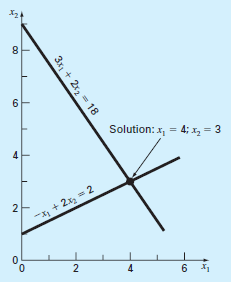
\includegraphics[width=0.3\linewidth]{fig_9_1}
    \caption{\textsf{Graphical solution of a set of two simultaneous linear algebraic equations. The intersection of the
    lines represents the solution.}}
    \label{fig:fig_9_1}
\end{figure}

\begin{figure}[H]
    \centering
    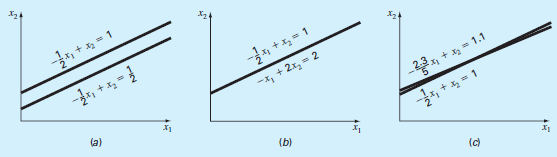
\includegraphics[width=0.7\linewidth]{fig_9_2}
    \caption{\textsf{Graphical depiction of singular and ill-conditioned systems: (a) no solution, (b) infinite solutions, and
    (c) ill-conditioned system where the slopes are so close that the point of intersection is difficult to detect visually.}}
    \label{fig:fig_9_2}
\end{figure}

\subsection{Determinants and Cramer's Rule}

Cramer's rule is another solution technique that is best suited to small numbers of equations. Before describing this method, we will briefly review the concept of the determinant, which is used to implement Cramer's rule. In addition, the determinant has relevance to the evaluation of the ill-conditioning of a matrix.
\medskip

\textbf{Determinants.} The determinant can be illustrated for a set of three equations:
$$
[A]\{x\}=\{b\}
$$
where $[A]$ is the coefficient matrix
$$
[A]=\left[\begin{array}{lll}
a_{11} & a_{12} & a_{13} \\
a_{21} & a_{22} & a_{23} \\
a_{31} & a_{32} & a_{33}
\end{array}\right]
$$
The determinant of this system is formed from the coefficients of [A] and is represented as
$$
D=\left|\begin{array}{lll}
a_{11} & a_{12} & a_{13} \\
a_{21} & a_{22} & a_{23} \\
a_{31} & a_{32} & a_{33}
\end{array}\right|
$$
Although the determinant $D$ and the coefficient matrix $[A]$ are composed of the same elements, they are completely different mathematical concepts. That is why they are distinguished visually by using brackets to enclose the matrix and straight lines to enclose the determinant. In contrast to a matrix, the determinant is a single number. For example, the value of the determinant for two simultaneous equations
$$
D=\left|\begin{array}{ll}
a_{11} & a_{12} \\
a_{21} & a_{22}
\end{array}\right|
$$
is calculated by
$$
D=a_{11} a_{22}-a_{12} a_{21}
$$
For the third-order case, the determinant can be computed as
$$
D=a_{11}\left|\begin{array}{ll}
a_{22} & a_{23} \\
a_{32} & a_{33}
\end{array}\right|-a_{12}\left|\begin{array}{ll}
a_{21} & a_{23} \\
a_{31} & a_{33}
\end{array}\right|+a_{13}\left|\begin{array}{ll}
a_{21} & a_{22} \\
a_{31} & a_{32}
\end{array}\right|
$$\hfill{(9.1)}
where the $2 \times 2$ determinants are called minors.

\begin{example} Determinants\\

    \noindent\textbf{Problem Statement.}\quad Compute values for the determinants of the systems represented in Figs. 9.1 and 9.2.\\

    \noindent\textbf{Solution.}\quad For Fig. 9.1:\\

    $$
    D=\left|\begin{array}{rr}
    3 & 2 \\
    -1 & 2
    \end{array}\right|=3(2)-2(-1)=8
    $$
    For Fig. 9.2a:
    $$
    D=\left|\begin{array}{ll}
    -\frac{1}{2} & 1 \\
    -\frac{1}{2} & 1
    \end{array}\right|=-\frac{1}{2}(1)-1\left(\frac{-1}{2}\right)=0
    $$
    For Fig. 9.2b:
    $$
    D=\left|\begin{array}{rr}
    -\frac{1}{2} & 1 \\
    -1 & 2
    \end{array}\right|=-\frac{1}{2}(2)-1(-1)=0
    $$
    For Fig. 9.2c:
    $$
    D=\left|\begin{array}{cc}
    -\frac{1}{2} & 1 \\
    -\frac{2.3}{5} & 1
    \end{array}\right|=-\frac{1}{2}(1)-1\left(\frac{-2.3}{5}\right)=-0.04
    $$

\end{example}

In the foregoing example, the singular systems had zero determinants. Additionally, the results suggest that the system that is almost singular (Fig. 9.2c) has a determinant that is close to zero. These ideas will be pursued further in our subsequent discussion of ill-conditioning in Chap. 11 .

Cramer's Rule. This rule states that each unknown in a system of linear algebraic equations may be expressed as a fraction of two determinants with denominator $D$ and with the numerator obtained from $D$ by replacing the column of coefficients of the unknown in question by the constants $b_{1}, b_{2}, \ldots, b_{n}$. For example, for three equations, $x_{1}$ would be computed as
$$
x_{1}=\frac{\left|\begin{array}{lll}
b_{1} & a_{12} & a_{13} \\
b_{2} & a_{22} & a_{23} \\
b_{3} & a_{32} & a_{33}
\end{array}\right|}{D}
$$

\begin{example} Cramer's Rule\\

    \noindent\textbf{Problem Statement.}\quad Use Cramer's rule to solve\\

    $$
    \begin{aligned}
    0.3 x_{1}+0.52 x_{2}+x_{3} &=-0.01 \\
    0.5 x_{1}+x_{2}+1.9 x_{3} &=0.67 \\
    0.1 x_{1}+0.3 x_{2}+0.5 x_{3} &=-0.44
    \end{aligned}
    $$


    \noindent\textbf{Solution.}\quad The determinant $D$ can be evaluated as [Eq. (9.1)]:\\

    $$
    D=0.3\left|\begin{array}{cc}
    1 & 1.9 \\
    0.3 & 0.5
    \end{array}\right|-0.52\left|\begin{array}{cc}
    0.5 & 1.9 \\
    0.1 & 0.5
    \end{array}\right|+1\left|\begin{array}{cc}
    0.5 & 1 \\
    0.1 & 0.3
    \end{array}\right|=-0.0022
    $$
    The solution can be calculated as
    $$
    x_{1}=\frac{\left|\begin{array}{ccc}
    -0.01 & 0.52 & 1 \\
    0.67 & 1 & 1.9 \\
    -0.44 & 0.3 & 0.5
    \end{array}\right|}{-0.0022}=\frac{0.03278}{-0.0022}=-14.9
    $$
    $$
    x_{2}=\frac{\left|\begin{array}{ccc}
    0.3 & -0.01 & 1 \\
    0.5 & 0.67 & 1.9 \\
    0.1 & -0.44 & 0.5
    \end{array}\right|}{-0.0022}=\frac{0.0649}{-0.0022}=-29.5
    $$
    $$
    x_{3}=\frac{\left|\begin{array}{ccc}
    0.3 & 0.52 & -0.01 \\
    0.5 & 1 & 0.67 \\
    0.1 & 0.3 & -0.44
    \end{array}\right|}{-0.0022}=\frac{-0.04356}{-0.0022}=19.8
    $$

\end{example}

\textbf{The det Function.} The determinant can be computed directly in MATLAB with the det function. For example, using the system from the previous example:

\begin{lstlisting}[numbers=none,frame=none]
    >> A=[0.3 0.52 1;0.5 1 1.9;0.1 0.3 0.5];
    >> D=det(A)
    D =
        -0.0022
\end{lstlisting}

Cramer's rule can be applied to compute $x_{1}$ as in

\begin{lstlisting}[numbers=none,frame=none]
    >> A(:,1)=[-0.01;0.67;-0.44]
    A =
        -0.0100 0.5200 1.0000
        0.6700 1.0000 1.9000
        -0.4400 0.3000 0.5000
    >> x1=det(A)/D
    x1 =
        -14.9000
\end{lstlisting}

For more than three equations, Cramer's rule becomes impractical because, as the number of equations increases, the determinants are time consuming to evaluate by hand (or by computer). Consequently, more efficient alternatives are used. Some of these alternatives are based on the last noncomputer solution technique covered in Section $9.1 .3$-the elimination of unknowns.

\subsection{Elimination of Unknowns}

The elimination of unknowns by combining equations is an algebraic approach that can be illustrated for a set of two equations:
\begin{center}
$a_{11} x_{1}+a_{12} x_{2}=b_{1}$ \hfill{(9.2)}

$a_{21} x_{1}+a_{22} x_{2}=b_{2}$ \hfill{(9.3)}
\end{center}

The basic strategy is to multiply the equations by constants so that one of the unknowns will be eliminated when the two equations are combined. The result is a single equation that can be solved for the remaining unknown. This value can then be substituted into either of the original equations to compute the other variable.
For example, Eq. (9.2) might be multiplied by $a_{21}$ and Eq. (9.3) by $a_{11}$ to give

\begin{center}
$a_{21} a_{11} x_{1}+a_{21} a_{12} x_{2}=a_{21} b_{1}$ \hfill{(9.4)}

$a_{11} a_{21} x_{1}+a_{11} a_{22} x_{2}=a_{11} b_{2}$ \hfill{(9.5)}
\end{center}

Subtracting Eq. (9.4) from Eq. (9.5) will, therefore, eliminate the $x_{1}$ term from the equations to yield
$$
a_{11} a_{22} x_{2}-a_{21} a_{12} x_{2}=a_{11} b_{2}-a_{21} b_{1}
$$
which can be solved for

$$
x_{2}=\frac{a_{11} b_{2}-a_{21} b_{1}}{a_{11} a_{22}-a_{21} a_{12}}
$$ \hfill{(9.6)}

Equation (9.6) can then be substituted into Eq. (9.2), which can be solved for
$$
x_{1}=\frac{a_{22} b_{1}-a_{12} b_{2}}{a_{11} a_{22}-a_{21} a_{12}}
$$\hfill{(9.7)}

Notice that Eqs. (9.6) and (9.7) follow directly from Cramer's rule:
$$
\begin{aligned}
x_{1} &=\frac{\left|\begin{array}{ll}
b_{1} & a_{12} \\
b_{2} & a_{22}
\end{array}\right|}{\left|\begin{array}{ll}
a_{11} & a_{12} \\
a_{21} & a_{22}
\end{array}\right|}=\frac{a_{22} b_{1}-a_{12} b_{2}}{a_{11} a_{22}-a_{21} a_{12}} \\
x_{2} &=\frac{\left|\begin{array}{ll}
a_{11} & b_{1} \\
a_{21} & b_{2}
\end{array}\right|}{\left|\begin{array}{ll}
a_{11} & a_{12} \\
a_{21} & a_{22}
\end{array}\right|}=\frac{a_{11} b_{2}-a_{21} b_{1}}{a_{11} a_{22}-a_{21} a_{12}}
\end{aligned}
$$
The elimination of unknowns can be extended to systems with more than two or three equations. However, the numerous calculations that are required for larger systems make the method extremely tedious to implement by hand. However, as described in Section $9.2$, the technique can be formalized and readily programmed for the computer.
\bigskip

\section{NAIVE GAUSS ELIMINATION}

In Section 9.1.3, the elimination of unknowns was used to solve a pair of simultaneous equations. The procedure consisted of two steps (Fig. 9.3):
1. The equations were manipulated to eliminate one of the unknowns from the equations. The result of this elimination step was that we had one equation with one unknown.
2. Consequently, this equation could be solved directly and the result back-substituted into one of the original equations to solve for the remaining unknown.

This basic approach can be extended to large sets of equations by developing a systematic scheme or algorithm to eliminate unknowns and to back-substitute. Gauss elimination is the most basic of these schemes.

This section includes the systematic techniques for forward elimination and back substitution that comprise Gauss elimination. Although these techniques are ideally suited for implementation on computers, some modifications will be required to obtain a reliable algorithm. In particular, the computer program must avoid division by zero. The following method is called "naive" Gauss elimination because it does not avoid this problem. Section $9.3$ will deal with the additional features required for an effective computer program.
The approach is designed to solve a general set of $n$ equations:
$$
\begin{aligned}
&a_{11} x_{1}+a_{12} x_{2}+a_{13} x_{3}+\cdots+a_{\ln } x_{n}=b_{1} \ \ \ \ \ \ \ \ \ \ (9.8a)\\
&a_{21} x_{1}+a_{22} x_{2}+a_{23} x_{3}+\cdots+a_{2 n} x_{n}=b_{2} \ \ \ \ \ \ \ \ \ \ (9.8b)\\
&\vdots \\
&\vdots \\
&a_{n 1} x_{1}+a_{n 2} x_{2}+a_{n 3} x_{3}+\cdots+a_{n n} x_{n}=b_{n} \ \ \ \ \ \ \ \ \ \ (9.8c)\\
\end{aligned}
$$

\begin{figure}[H]
    \centering
    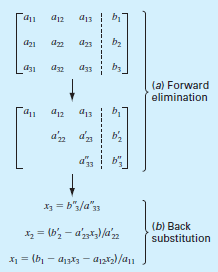
\includegraphics[width=0.4\linewidth]{fig_9_3}
    \caption{\textsf{The two phases of Gauss elimination: (a) forward elimination and (b) back substitution.}}
    \label{fig:fig_9_3}
\end{figure}

As was the case with the solution of two equations, the technique for $n$ equations consists of two phases: elimination of unknowns and solution through back substitution.
\bigskip

\noindent\textbf{Forward Elimination of Unknowns.} The first phase is designed to reduce the set of equations to an upper triangular system (Fig. 9.3a). The initial step will be to eliminate the first unknown $x_{1}$ from the second through the $n$th equations. To do this, multiply Eq. (9.8a) by $a_{21} / a_{11}$ to give
\bigskip

$a_{21} x_{1}+\frac{a_{21}}{a_{11}} a_{12} x_{2}+\frac{a_{21}}{a_{11}} a_{13} x_{3}+\cdots+\frac{a_{21}}{a_{11}} a_{1 n} x_{n}=\frac{a_{21}}{a_{11}} b_{1}$ \hfill{(9.9)}
\bigskip

This equation can be subtracted from Eq. (9.8b) to give \bigskip

$\left(a_{22}-\frac{a_{21}}{a_{11}} a_{12}\right) x_{2}+\cdots+\left(a_{2 n}-\frac{a_{21}}{a_{11}} a_{1 n}\right) x_{n}=b_{2}-\frac{a_{21}}{a_{11}} b_{1} $ \bigskip

or\bigskip

$a_{22}^{\prime} x_{2}+\cdots+a_{2 n}^{\prime} x_{n}=b_{2}^{\prime}$\bigskip

\noindent where the prime indicates that the elements have been changed from their original values.

The procedure is then repeated for the remaining equations. For instance, Eq. (9.8a) can be multiplied by $a_{31} / a_{11}$ and the result subtracted from the third equation. Repeating the procedure for the remaining equations results in the following modified system:


$$
\begin{aligned}
&a_{11} x_{1}+a_{12} x_{2}+a_{13} x_{3}+\cdots+a_{1 n} x_{n}=b_{1} \ \ \ \ \ \ \ \ \ \ (9.10a)\\
&a_{22}^{\prime} x_{2}+a_{23}^{\prime} x_{3}+\cdots+a_{2 n}^{\prime} x_{n}=b_{2}^{\prime} \ \ \ \ \ \ \ \ \ \ (9.10b)\\
&a_{32}^{\prime} x_{2}+a_{33}^{\prime} x_{3}+\cdots+a_{3 n}^{\prime} x_{n}=b_{3}^{\prime} \ \ \ \ \ \ \ \ \ \ (9.10c)\\
&\vdots \\
&a_{n 2}^{\prime} x_{2}+a_{n 3}^{\prime} x_{3}+\cdots+a_{n n}^{\prime} x_{n}=b_{n}^{\prime} \ \ \ \ \ \ \ \ \ \ (9.10d)\\
\end{aligned}
$$

For the foregoing steps, Eq. $(9.8 a)$ is called the pivot equation and $a_{11}$ is called the pivot element. Note that the process of multiplying the first row by $a_{21} / a_{11}$ is equivalent to dividing it by $a_{11}$ and multiplying it by $a_{21}$. Sometimes the division operation is referred to as normalization. We make this distinction because a zero pivot element can interfere with normalization by causing a division by zero. We will return to this important issue after we complete our description of naive Gauss elimination.

The next step is to eliminate $x_{2}$ from Eq. $(9.10 c)$ through $(9.10 d)$. To do this, multiply Eq. (9.10b) by $a_{32}^{\prime} / a_{22}^{\prime}$ and subtract the result from Eq. (9.10c). Perform a similar elimination for the remaining equations to yield
$$
\begin{array}{r}
a_{11} x_{1}+a_{12} x_{2}+a_{13} x_{3}+\cdots+a_{1 n} x_{n}=b_{1} \\
a_{22}^{\prime} x_{2}+a_{23}^{\prime} x_{3}+\cdots+a_{2 n}^{\prime} x_{n}=b_{2}^{\prime} \\
a_{33}^{\prime \prime} x_{3}+\cdots+a_{3 n}^{\prime \prime} x_{n}=b_{3}^{\prime \prime} \\
\vdots \\
a_{n 3}^{\prime \prime} x_{3}+\cdots+a_{n n}^{\prime} x_{n}=b_{n}^{\prime \prime}
\end{array}
$$
where the double prime indicates that the elements have been modified twice.
The procedure can be continued using the remaining pivot equations. The final manipulation in the sequence is to use the $(n-1)$ th equation to eliminate the $x_{n-1}$ term from the $n$th equation. At this point, the system will have been transformed to an upper triangular system:
$$
\begin{aligned}
a_{11} x_{1}+a_{12} x_{2}+a_{13} x_{3}+\cdots+a_{1 n} x_{n} &=b_{1} \ \ \ \ \ \ \ \ \ \ (9.11a)\\
a_{22}^{\prime} x_{2}+a_{23}^{\prime} x_{3}+\cdots+a_{2 n}^{\prime} x_{n} &=b_{2}^{\prime} \ \ \ \ \ \ \ \ \ \ (9.11b)\\
a_{33}^{\prime \prime} x_{3}+\cdots+a_{3 n}^{\prime \prime} x_{n} &=b_{3}^{\prime \prime} \ \ \ \ \ \ \ \ \ \ (9.11c)\\
\ddots & \vdots \\
a_{n n}^{(n-1)} x_{n} &=b_{n}^{(n-1)} \ \ \ \ \ \ \ \  (9.11d)\\
\end{aligned}
$$

\noindent \textbf{Back Substitution.} Equation $(9.11 d)$ can now be solved for $x_{n}$ :
$$
x_{n}=\frac{b_{n}^{(n-1)}}{a_{n n}^{(n-1)}}
$$\hfill{(9.12)}

This result can be back-substituted into the $(n-1)$ th equation to solve for $x_{n-1}$. The procedure, which is repeated to evaluate the remaining $x$ 's, can be represented by the following formula:
$$
x_{i}=\frac{b_{i}^{(i-1)}-\sum_{j=i+1}^{n} a_{i j}^{(i-1)} x_{j}}{a_{i i}^{(i-1)}} \quad \text { for } i=n-1, n-2, \ldots, 1
$$\hfill{(9.13)}

\begin{example} Naive Gauss Elimination\\

    \noindent\textbf{Problem Statement.}\quad Use Gauss elimination to solve\\

    $$
    \begin{aligned}
    3 x_{1}-0.1 x_{2}-0.2 x_{3} &=7.85  \ \ \ \ \ \ \ \ \ \ (E9.3.1)\\
    0.1 x_{1}+7 x_{2}-0.3 x_{3} &=-19.3  \ \ \ \ \ \ \ \ \ \ (E9.3.2)\\
    0.3 x_{1}-0.2 x_{2}+10 x_{3} &=71.4  \ \ \ \ \ \ \ \ \ \ (E9.3.3)\\
    \end{aligned}
    $$

    \noindent\textbf{Solution.}\quad The first part of the procedure is forward elimination. Multiply Eq. (E9.3.1) by $0.1 / 3$ and subtract the result from Eq. (E9.3.2) to give\\
    $$
    7.00333 x_{2}-0.293333 x_{3}=-19.5617
    $$
    Then multiply Eq. (E9.3.1) by $0.3 / 3$ and subtract it from Eq. (E9.3.3). After these operations, the set of equations is
    $$
    \begin{aligned}
    3 x_{1}-\quad 0.1 x_{2}-\quad 0.2 x_{3} &=7.85  \ \ \ \ \ \ \ \ \ \ (E9.3.4)\\
    7.00333 x_{2}-0.293333 x_{3} &=-19.5617  \ \ \ \ \ \ \ \ \ \ (E9.3.5)\\
    -0.190000 x_{2}+10.0200 x_{3} &=70.6150  \ \ \ \ \ \ \ \ \ \ (E9.3.6)\\
    \end{aligned}
    $$
    To complete the forward elimination, $x_{2}$ must be removed from Eq. (E9.3.6). To accomplish this, multiply Eq. (E9.3.5) by $-0.190000 / 7.00333$ and subtract the result from Eq. (E9.3.6). This eliminates $x_{2}$ from the third equation and reduces the system to an upper triangular form, as in
    $$
    \begin{aligned}
    3 x_{1}-0.1 x_{2}-\quad 0.2 x_{3} &=7.85   \ \ \ \ \ \ \ \ \ \ (E9.3.7)\\
    7.00333 x_{2}-0.293333 x_{3} &=-19.5617   \ \ \ \ \ \ \ \ \ \ (E9.3.8)\\
    10.0120 x_{3} &=70.0843   \ \ \ \ \ \ \ \ \ \ (E9.3.9)\\
    \end{aligned}
    $$
    We can now solve these equations by back substitution. First, Eq. (E9.3.9) can be solved for
    $$
    x_{3}=\frac{70.0843}{10.0120}=7.00003
    $$
    This result can be back-substituted into Eq. (E9.3.8), which can then be solved for
    $$
    x_{2}=\frac{-19.5617+0.293333(7.00003)}{7.00333}=-2.50000
    $$
    Finally, $x_{3}=7.00003$ and $x_{2}=-2.50000$ can be substituted back into Eq. (E9.3.7), which can be solved for
    $$
    x_{1}=\frac{7.85+0.1(-2.50000)+0.2(7.00003)}{3}=3.00000
    $$
    Although there is a slight round-off error, the results are very close to the exact solution of $x_{1}=3, x_{2}=-2.5$, and $x_{3}=7$. This can be verified by substituting the results into the original equation set:
    $$
    \begin{aligned}
    &3(3)-0.1(-2.5)-0.2(7.00003)=7.84999 \cong 7.85 \\
    &0.1(3)+7(-2.5)-0.3(7.00003)=-19.30000=-19.3 \\
    &0.3(3)-0.2(-2.5)+10(7.00003)=71.4003 \cong 71.4
    \end{aligned}
    $$

\end{example}

\begin{lstlisting}[numbers=none,frame=none]
    function x = GaussNaive(A,b)
    % GaussNaive: naive Gauss elimination
    % x = GaussNaive(A,b): Gauss elimination without pivoting.
    % input:
    % A = coefficient matrix
    % b = right hand side vector
    % output:
    % x = solution vector
    [m,n] = size(A);
    if m~=n, error('Matrix A must be square'); end
    nb = n+1;
    Aug = [A b];
    % forward elimination
    for k = 1:n-1
    for i = k+1:n
    factor = Aug(i,k)/Aug(k,k);
    Aug(i,k:nb) = Aug(i,k:nb)-factor*Aug(k,k:nb);
    end
    end
    % back substitution
    x = zeros(n,1);
    x(n) = Aug(n,nb)/Aug(n,n);
    for i = n-1:-1:1
    x(i) = (Aug(i,nb)-Aug(i,i+1:n)*x(i+1:n))/Aug(i,i);
    end
\end{lstlisting}
\begin{figure}[H]
    \centering
    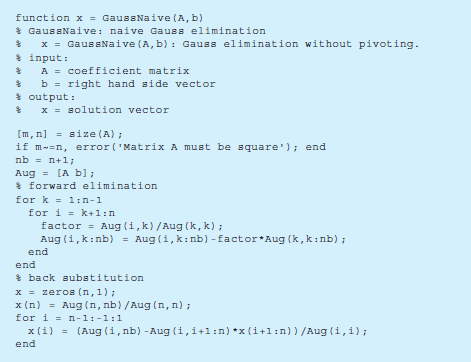
\includegraphics[width=0.000001\linewidth]{fig_9_4}
    \caption{\textsf{An M-file to implement naive Gauss elimination.}}
    \label{fig:fig_9_4}
\end{figure}

\subsection{MATLAB M-file: \texttt{GaussNaive}}
An M-file that implements naive Gauss elimination is listed in Fig. 9.4. Notice that the coefficient matrix A and the right-hand-side vector $\mathrm{b}$ are combined in the augmented matrix Aug. Thus, the operations are performed on Aug rather than separately on A and $\mathrm{b}$.
Two nested loops provide a concise representation of the forward elimination step. An outer loop moves down the matrix from one pivot row to the next. The inner loop moves below the pivot row to each of the subsequent rows where elimination is to take place. Finally, the actual elimination is represented by a single line that takes advantage of MATLAB's ability to perform matrix operations.

The back-substitution step follows directly from Eqs. (9.12) and (9.13). Again, MATLAB's ability to perform matrix operations allows Eq. (9.13) to be programmed as a single line.

\subsection{Operation Counting}
The execution time of Gauss elimination depends on the amount of floating-point operations (or flops) involved in the algorithm. On modern computers using math coprocessors, the time consumed to perform addition/subtraction and multiplication/division is about the same.

\noindent Therefore, totaling up these operations provides insight into which parts of the algorithm are most time consuming and how computation time increases as the system gets larger.

Before analyzing naive Gauss elimination, we will first define some quantities that facilitate operation counting:
$$
\begin{aligned}
&\sum_{i=1}^{m} c f(i)=c \sum_{i=1}^{m} f(i) \sum_{i=1}^{m} f(i)+g(i)=\sum_{i=1}^{m} f(i)+\sum_{i=1}^{m} g(i)   \ \ \ \ \ \ \ \ \ \ (9.14a,b)\\
&\sum_{i=1}^{m} 1=1+1+1+\cdots+1=m \sum_{i=k}^{m} 1=m-k+1   \ \ \ \ \ \ \ \ \ \ (9.14c,d)\\
&\sum_{i=1}^{m} i=1+2+3+\cdots+m=\frac{m(m+1)}{2}=\frac{m^{2}}{2}+O(m)   \ \ \ \ \ \ \ \ \ \ (9.14e)\\
&\sum_{i=1}^{m} i^{2}=1^{2}+2^{2}+3^{2}+\cdots+m^{2}=\frac{m(m+1)(2 m+1)}{6}=\frac{m^{3}}{3}+O\left(m^{2}\right)   \ \ \ \ \ \ \ \ \ \ (9.14f)\\
\end{aligned}
$$
where $O\left(m^{n}\right)$ means "terms of order $m^{n}$ and lower."
Now let us examine the naive Gauss elimination algorithm (Fig. 9.4) in detail. We will first count the flops in the elimination stage. On the first pass through the outer loop, $k=1$. Therefore, the limits on the inner loop are from $i=2$ to $n$. According to Eq. $(9.14 d)$, this means that the number of iterations of the inner loop will be
\bigskip

$\sum_{i=2}^{n} 1=n-2+1=n-1$ \hfill{(9.15)}\bigskip

\noindent For every one of these iterations, there is one division to calculate the factor. The next line then performs a multiplication and a subtraction for each column element from 2 to $n b$. Because $n b=n+1$, going from 2 to $n b$ results in $n$ multiplications and $n$ subtractions. Together with the single division, this amounts to $n+1$ multiplications/divisions and $n$ addition/subtractions for every iteration of the inner loop. The total for the first pass through the outer loop is therefore $(n-1)(n+1)$ multiplication/divisions and $(n-1)(n)$ addition/subtractions.

Similar reasoning can be used to estimate the flops for the subsequent iterations of the outer loop. These can be summarized as
\bigskip

\begin{tabular}{cccc}
\hline Outer Loop $k$ & Inner Loop $i$ & Addition/Subtraction Flops & Multiplication/Division Flops \\
\hline 1 & $2, n$ & $(n-1)(n)$ & $(n-1)(n+1)$ \\
2 & $3, n$ & $(n-2) (n-1)$ & $(n-2)(n)$ \\
$\vdots$ & $\vdots$ & & \\
$k$ & $k + 1, n$ & $(n-k)(n+1-k)$& $(n-k)(n+2-k)$ \\
$\vdots$ & $\vdots$ & & \\
$n-1$ & $n,n$ & (1)(2) & (1)(3)
\end{tabular}\bigskip


\noindent Therefore, the total addition/subtraction flops for elimination can be computed as \bigskip

$\sum_{k=1}^{n-1}(n-k)(n+1-k)=\sum_{k=1}^{n-1}\left[n(n+1)-k(2 n+1)+k^{2}\right]$ \hfill{(9.16)}
\bigskip

Or
$$
n(n+1) \sum_{k=1}^{n-1} 1-(2 n+1) \sum_{k=1}^{n-1} k+\sum_{k=1}^{n-1} k^{2}
$$\hfill{(9.17)}

Applying some of the relationships from Eq. (9.14) yields
$$
\left[n^{3}+O(n)\right]-\left[n^{3}+O\left(n^{2}\right)\right]+\left[\frac{1}{3} n^{3}+O\left(n^{2}\right)\right]=\frac{n^{3}}{3}+O(n)
$$\hfill{(9.18)}

A similar analysis for the multiplication/division flops yields
$$
\left[n^{3}+O\left(n^{2}\right)\right]-\left[n^{3}+O(n)\right]+\left[\frac{1}{3} n^{3}+O\left(n^{2}\right)\right]=\frac{n^{3}}{3}+O\left(n^{2}\right)
$$\hfill{(9.19)}

Summing these results gives
$$
\frac{2 n^{3}}{3}+O\left(n^{2}\right)
$$\hfill{(9.20)}

Thus, the total number of flops is equal to $2 n^{3} / 3$ plus an additional component proportional to terms of order $n^{2}$ and lower. The result is written in this way because as $n$ gets large, the $O\left(n^{2}\right)$ and lower terms become negligible. We are therefore justified in concluding that for large $n$, the effort involved in forward elimination converges on $2 n^{3} / 3$.

Because only a single loop is used, back substitution is much simpler to evaluate. The number of addition/subtraction flops is equal to $n(n-1) / 2$. Because of the extra division prior to the loop, the number of multiplication/division flops is $n(n+1) / 2$. These can be added to arrive at a total of
$$
n^{2}+O(n)
$$\hfill{(9.21)}

Thus, the total effort in naive Gauss elimination can be represented as\bigskip

$\frac{2 n^{3}}{3}+O\left(n^{2}\right)+n^{2}+O(n) \stackrel{\text { as } n \text { increases }}{\longrightarrow} \frac{2 n^{3}}{3}+O\left(n^{2}\right)$\hfill{(9.22)}
\bigskip

Two useful general conclusions can be drawn from this analysis:

1. As the system gets larger, the computation time increases greatly. As in Table 9.1, the amount of flops increases nearly three orders of magnitude for every order of magnitude increase in the number of equations.

TABLE $9.1$ Number of flops for naive Gauss elimination.

\begin{tabular}{rccccc}
$n$ & Elimination & Back Substitution & Total Flops & $\mathbf{2 n ^ { 3 } / 3}$ & Percent Due to Elimination \\
\hline 10 & 705 & 100 & 805 & 667 & $87.58 \%$ \\
100 & 671550 & 10000 & 681550 & 666667 & $98.53 \%$ \\
1000 & $6.67 \times 10^{8}$ & $1 \times 10^{6}$ & $6.68 \times 10^{8}$ & $6.67 \times 10^{9}$ & $99.85 \%$ \\
\hline
\end{tabular}
\bigskip

2. Most of the effort is incurred in the elimination step. Thus, efforts to make the method more efficient should probably focus on this step.
\bigskip

\section{PIVOTING}
\label{sec:sec_9_3}

The primary reason that the foregoing technique is called "naive" is that during both the elimination and the back-substitution phases, it is possible that a division by zero can occur. For example, if we use naive Gauss elimination to solve
$$
\begin{aligned}
2 x_{2}+3 x_{3} &=8 \\
4 x_{1}+6 x_{2}+7 x_{3} &=-3 \\
2 x_{1}-3 x_{2}+6 x_{3} &=5
\end{aligned}
$$
the normalization of the first row would involve division by $a_{11}=0$. Problems may also arise when the pivot element is close, rather than exactly equal, to zero because if the magnitude of the pivot element is small compared to the other elements, then round-off errors can be introduced.

Therefore, before each row is normalized, it is advantageous to determine the coefficient with the largest absolute value in the column below the pivot element. The rows can then be switched so that the largest element is the pivot element. This is called partial pivoting.

If columns as well as rows are searched for the largest element and then switched, the procedure is called complete pivoting. Complete pivoting is rarely used because most of the improvement comes from partial pivoting. In addition, switching columns changes the order of the $x$ 's and, consequently, adds significant and usually unjustified complexity to the computer program.

The following example illustrates the advantages of partial pivoting. Aside from avoiding division by zero, pivoting also minimizes round-off error. As such, it also serves as a partial remedy for ill-conditioning.

\begin{example} Partial Pivoting\\

    \noindent\textbf{Problem Statement.}\quad Use Gauss elimination to solve\\

    $$
    \begin{aligned}
    &0.0003 x_{1}+3.0000 x_{2}=2.0001 \\
    &1.0000 x_{1}+1.0000 x_{2}=1.0000
    \end{aligned}
    $$
    Note that in this form the first pivot element, $a_{11}=0.0003$, is very close to zero. Then repeat the computation, but partial pivot by reversing the order of the equations. The exact solution is $x_{1}=1 / 3$ and $x_{2}=2 / 3$.

    \noindent\textbf{Solution.}\quad Multiplying the first equation by $1 /(0.0003)$ yields\\

    $$
    x_{1}+10,000 x_{2}=6667
    $$
    which can be used to eliminate $x_{1}$ from the second equation:
    $$
    -9999 x_{2}=-6666
    $$
    which can be solved for $x_{2}=2 / 3$. This result can be substituted back into the first equation to evaluate $x_{1}$ :
    $$
    x_{1}=\frac{2.0001-3(2 / 3)}{0.0003}
    $$

    Due to subtractive cancellation, the result is very sensitive to the number of significant figures carried in the computation:
    \bigskip

    \begin{tabular}{cccc}
    \hline Signlficant Figures & $x_{2}$ & $x_{1}$ & Absolute Value of Percent Relative Error for $x_{1}$ \\
    \hline 3 & $0.667$ & $-3.33$ & 1099 \\
    4 & $0.6667$ & $0.0000$ & 100 \\
    5 & $0.66667$ & $0.30000$ & 10 \\
    6 & $0.666667$ & $0.330000$ & 1 \\
    7 & $0.6666667$ & $0.3330000$ & $0.1$ \\
    \hline
    \end{tabular}
    \bigskip

    Note how the solution for $x_{1}$ is highly dependent on the number of significant figures. This is because in Eq. (E9.4.1), we are subtracting two almost-equal numbers.

    On the other hand, if the equations are solved in reverse order, the row with the larger pivot element is normalized. The equations are
    \bigskip

    $$
    \begin{aligned}
    &1.0000 x_{1}+1.0000 x_{2}=1.0000 \\
    &0.0003 x_{1}+3.0000 x_{2}=2.0001
    \end{aligned}
    $$
    \bigskip

    Elimination and substitution again yields $x_{2}=2 / 3$. For different numbers of significant figures, $x_{1}$ can be computed from the first equation, as in

    $$
    x_{1}=\frac{1-(2 / 3)}{1}
    $$

    This case is much less sensitive to the number of significant figures in the computation:
    \bigskip

    \begin{tabular}{clcc}
    Significant Figgures & \multicolumn{1}{c}{$x_{2}$} & \multicolumn{1}{c}{$x_{1}$} & \multicolumn{1}{c}{ Absolute Value of Percent Relative Error for $x_{1}$} \\
    \hline 3 & $0.667$ & $0.333$ & $0.1$ \\
    4 & $0.6667$ & $0.3333$ & $0.01$ \\
    5 & $0.66667$ & $0.33333$ & $0.001$ \\
    6 & $0.666667$ & $0.333333$ & $0.0001$ \\
    7 & $0.6666667$ & $0.3333333$ & $0.0000$
    \end{tabular}
    \bigskip

    Thus, a pivot strategy is much more satisfactory.

\end{example}

\subsection{MATLAB M-file: \texttt{Gausspivot}}

An M-file that implements Gauss elimination with partial pivoting is listed in Fig. 9.5. It is identical to the M-file for naive Gauss elimination presented previously in Section 9.2.1 with the exception of the bold portion that implements partial pivoting.

Notice how the built-in MATLAB function max is used to determine the largest available coefficient in the column below the pivot element. The max function has the syntax

\begin{lstlisting}[numbers=none,frame=none]
    [y, 1]=\max (x)
\end{lstlisting}

where $y$ is the largest element in the vector $x$, and $i$ is the index corresponding to that element.

\begin{lstlisting}[numbers=none,frame=none]
    function x = GaussPivot(A,b)
    % GaussPivot: Gauss elimination pivoting
    % x = GaussPivot(A,b): Gauss elimination with pivoting.
    % input:
    % A = coefficient matrix
    % b = right hand side vector
    % output:
    % x = solution vector
    [m,n]=size(A);
    if m~=n, error('Matrix A must be square'); end
    nb=n+1;
    Aug=[A b];
    % forward elimination
    for k = 1:n-1
    % partial pivoting
    [big,i]=max(abs(Aug(k:n,k)));
    ipr=i+k-1;
    if ipr~=k
    Aug([k,ipr],:)=Aug([ipr,k],:);
    end
    for i = k+1:n
    factor=Aug(i,k)/Aug(k,k);
    Aug(i,k:nb)=Aug(i,k:nb)-factor*Aug(k,k:nb);
    end
    end
    % back substitution
    x=zeros(n,1);
    x(n)=Aug(n,nb)/Aug(n,n);
    for i = n-1:-1:1
    x(i)=(Aug(i,nb)-Aug(i,i+1:n)*x(i+1:n))/Aug(i,i);
    end
\end{lstlisting}
\begin{figure}[H]
    \centering
    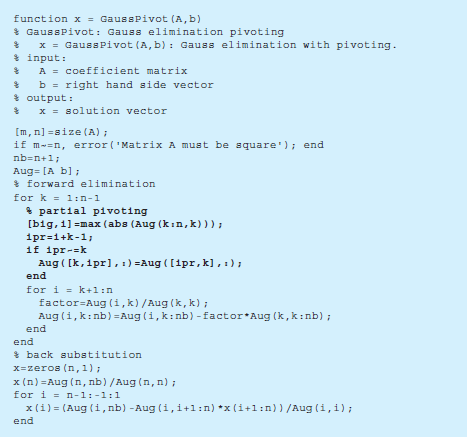
\includegraphics[width=0.000001\linewidth]{fig_9_5}
    \caption{\textsf{An M-file to implement Gauss elimination with partial pivoting.}}
    \label{fig:fig_9_5}
\end{figure}

\subsection{Determinant Evaluation with Gauss Elimination}

At the end of Sec. 9.1.2, we suggested that determinant evaluation by expansion of minors was impractical for large sets of equations. However, because the determinant has value in assessing system condition, it would be useful to have a practical method for computing this quantity.

Fortunately, Gauss elimination provides a simple way to do this. The method is based on the fact that the determinant of a triangular matrix can be simply computed as the product of its diagonal elements:
$$
D=a_{11} a_{22} a_{33} \cdots a_{n n}
$$
The validity of this formulation can be illustrated for a $3 \times 3$ system:
$$
D=\left|\begin{array}{ccc}
a_{11} & a_{12} & a_{13} \\
0 & a_{22} & a_{23} \\
0 & 0 & a_{33}
\end{array}\right|
$$
where the determinant can be evaluated as [recall Eq. (9.1)]:
$$
D=a_{11}\left|\begin{array}{cc}
a_{22} & a_{23} \\
0 & a_{33}
\end{array}\right|-a_{12}\left|\begin{array}{cc}
0 & a_{23} \\
0 & a_{33}
\end{array}\right|+a_{13}\left|\begin{array}{cc}
0 & a_{22} \\
0 & 0
\end{array}\right|
$$
or, by evaluating the minors:
$$
D=a_{11} a_{22} a_{33}-a_{12}(0)+a_{13}(0)=a_{11} a_{22} a_{33}
$$
Recall that the forward-elimination step of Gauss elimination results in an upper triangular system. Because the value of the determinant is not changed by the forwardelimination process, the determinant can be simply evaluated at the end of this step via
$$
D=a_{11} a_{22}^{\prime} a_{33}^{\prime \prime} \cdots a_{n A}^{(n-1)}
$$
where the superscripts signify the number of times that the elements have been modified by the elimination process. Thus, we can capitalize on the effort that has already been expended in reducing the system to triangular form and, in the bargain, come up with a simple estimate of the determinant.

There is a slight modification to the above approach when the program employs partial pivoting. For such cases, the determinant changes sign every time a row is switched. One way to represent this is by modifying the determinant calculation as in
$$
D=a_{11} a_{22}^{\prime} a_{33}^{\prime \prime} \cdots a_{n \pi}^{(n-1)}(-1)^{p}
$$
where $p$ represents the number of times that rows are pivoted. This modification can be incorporated simply into a program by merely keeping track of the number of pivots that take place during the course of the computation.
\bigskip

\section{TRIDIAGONAL SYSTEMS}
\label{sec:sec_8_4}

Certain matrices have a particular structure that can be exploited to develop efficient solution schemes. For example, a banded matrix is a square matrix that has all elements equal to zero, with the exception of a band centered on the main diagonal.
A tridiagonal system has a bandwidth of 3 and can be expressed generally as
\bigskip

$\left[\begin{array}{cccccccc}f_{1} & g_{1} & & & & & & \\ e_{2} & f_{2} & g_{2} & & & & & \\ & e_{3} & f_{3} & g_{3} & & & & \\ & & \cdot & \cdot & \cdot & & & \\ & & & \cdot & \cdot & \cdot & & \\ & & & & \cdot & \cdot & \cdot & \\ & & & & & e_{n-1} & f_{n-1} & g_{n-1} \\ & & & & & & e_{n} & f_{n}\end{array}\right]\left\{\begin{array}{c}x_{1} \\ x_{2} \\ x_{3} \\ \cdot \\ \cdot \\ x_{n-1} \\ x_{n}\end{array}\right\}=\left\{\begin{array}{c}r_{1} \\ r_{2} \\ r_{3} \\ \cdot \\ \cdot \\ \cdot \\ r_{n-1} \\ r_{n}\end{array}\right\}$ \hfill{9.23}

\bigskip
Notice that we have changed our notation for the coefficients from $a$ 's and $b$ 's to $e$ 's, $f$ 's, $g$ 's, and $r$ 's. This was done to avoid storing large numbers of useless zeros in the square matrix of $a$ 's. This space-saving modification is advantageous because the resulting algorithm requires less computer memory.

An algorithm to solve such systems can be directly patterned after Gauss eliminationthat is, using forward elimination and back substitution. However, because most of the matrix elements are already zero, much less effort is expended than for a full matrix. This efficiency is illustrated in the following example.

\begin{example} Solution of a Tridiagonal System\\

    \noindent\textbf{Problem Statement.}\quad Solve the following tridiagonal system:\\

    $$
    \left[\begin{array}{cccc}
    2.04 & -1 & & \\
    -1 & 2.04 & -1 & \\
    & -1 & 2.04 & -1 \\
    & & -1 & 2.04
    \end{array}\right]\left\{\begin{array}{l}
    x_{1} \\
    x_{2} \\
    x_{3} \\
    x_{4}
    \end{array}\right\}=\left\{\begin{array}{c}
    40.8 \\
    0.8 \\
    0.8 \\
    200.8
    \end{array}\right\}
    $$

    \noindent\textbf{Solution.}\quad As with Gauss elimination, the first step involves transforming the matrix to upper triangular form. This is done by multiplying the first equation by the factor $e_{2} / f_{1}$ and subtracting the result from the second equation. This creates a zero in place of $e_{2}$ and transforms the other coefficients to new values,\\

    $$
    \begin{aligned}
    f_{2} &=f_{2}-\frac{e_{2}}{f_{1}} g_{1}=2.04-\frac{-1}{2.04}(-1)=1.550 \\
    r_{2} &=r_{2}-\frac{e_{2}}{f_{1}} r_{1}=0.8-\frac{-1}{2.04}(40.8)=20.8
    \end{aligned}
    $$
    Notice that $g_{2}$ is unmodified because the element above it in the first row is zero.
    After performing a similar calculation for the third and fourth rows, the system is transformed to the upper triangular form
    $$
    \left[\begin{array}{cccc}
    2.04 & -1 & & \\
    & 1.550 & -1 & \\
    & & 1.395 & -1 \\
    & & & 1.323
    \end{array}\right]\left\{\begin{array}{l}
    x_{1} \\
    x_{2} \\
    x_{3} \\
    x_{4}
    \end{array}\right\}=\left\{\begin{array}{c}
    40.8 \\
    20.8 \\
    14.221 \\
    210.996
    \end{array}\right\}
    $$
    Now back substitution can be applied to generate the final solution:
    $$
    \begin{aligned}
    &x_{4}=\frac{r_{4}}{f_{4}}=\frac{210.996}{1.323}=159.480 \\
    &x_{3}=\frac{r_{3}-g_{3} x_{4}}{f_{3}}=\frac{14.221-(-1) 159.480}{1.395}=124.538 \\
    &x_{2}=\frac{r_{2}-g_{2} x_{3}}{f_{2}}=\frac{20.800-(-1) 124.538}{1.550}=93.778 \\
    &x_{1}=\frac{r_{1}-g_{1} x_{2}}{f_{1}}=\frac{40.800-(-1) 93.778}{2.040}=65.970
    \end{aligned}
    $$

\end{example}

\begin{lstlisting}[numbers=none,frame=none]
    function x = Tridiag(e,f,g,r)
    % Tridiag: Tridiagonal equation solver banded system
    % x = Tridiag(e,f,g,r): Tridiagonal system solver.
    % input:
    % e = subdiagonal vector
    % f = diagonal vector
    % g = superdiagonal vector
    % r = right hand side vector
    % output:
    % x = solution vector
    n=length(f);
    % forward elimination
    for k = 2:n
    factor = e(k)/f(k-1);
    f(k) = f(k) - factor*g(k-1);
    r(k) = r(k) - factor*r(k-1);
    end
    % back substitution
    x(n) = r(n)/f(n);
    for k = n-1:-1:1
    x(k) = (r(k)-g(k)*x(k+1))/f(k);
    end
\end{lstlisting}
\begin{figure}[H]
    \centering
    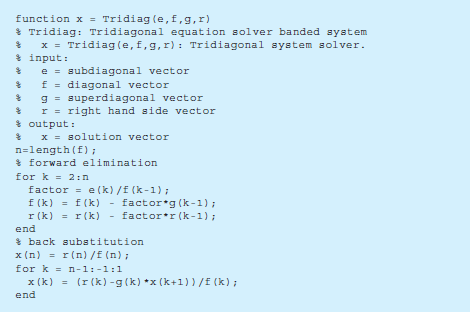
\includegraphics[width=0.000001\linewidth]{fig_9_6}
    \caption{\textsf{An M-file to solve a tridiagonal system.}}
    \label{fig:fig_9_6}
\end{figure}

\subsection{MATLAB M-file: \texttt{Tridiag}}

An M-file that solves a tridiagonal system of equations is listed in Fig. 9.6. Note that the algorithm does not include partial pivoting. Although pivoting is sometimes required, most tridiagonal systems routinely solved in engineering and science do not require pivoting.
Recall that the computational effort for Gauss elimination was proportional to $n^{3}$. Because of its sparseness, the effort involved in solving tridiagonal systems is proportional to $n$. Consequently, the algorithm in Fig. $9.6$ executes much, much faster than Gauss elimination, particularly for large systems.
\\

\section{\textbf{CASE STUDY} - MODEL OF A HEATED ROD}

\textbf{Background.} Linear algebraic equations can arise when modeling distributed systems. For example, Fig. $9.7$ shows a long, thin rod positioned between two walls that are held at constant temperatures. Heat flows through the rod as well as between the rod and the surrounding air. For the steady-state case, a differential equation based on heat conservation can be written for such a system as

$$
\frac{d^{2} T}{d x^{2}}+h^{\prime}\left(T_{a}-T\right)=0
$$ \hfill{(9.24)}

\begin{figure}[H]
    \centering
    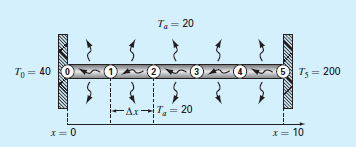
\includegraphics[width=0.5\linewidth]{fig_9_7}
    \caption{\textsf{A noninsulated uniform rod positioned between two walls of constant but different temperature.
    The finite-difference representation employs four interior nodes.}}
    \label{fig:fig_9_7}
\end{figure}

where $T=$ temperature $\left({ }^{\circ} \mathrm{C}\right), x=$ distance along the $\operatorname{rod}(\mathrm{m}), h^{\prime}=$ a heat transfer coefficient between the rod and the surrounding air $\left(\mathrm{m}^{-2}\right)$, and $T_{a}=$ the air temperature $\left({ }^{\circ} \mathrm{C}\right)$.

Given values for the parameters, forcing functions, and boundary conditions, calculus can be used to develop an analytical solution. For example, if $h^{\prime}=0.01, T_{a}=20, T(0)=$ 40 , and $T(10)=200$, the solution is
$$
T=73.4523 e^{0.1 x}-53.4523 e^{-0.1 x}+20
$$ \hfill{9.25}

Although it provided a solution here, calculus does not work for all such problems. In such instances, numerical methods provide a valuable alternative. In this case study, we will use finite differences to transform this differential equation into a tridiagonal system of linear algebraic equations which can be readily solved using the numerical methods described in this chapter.

\noindent\textbf{Solution.} Equation (9.24) can be transformed into a set of linear algebraic equations by conceptualizing the rod as consisting of a series of nodes. For example, the rod in Fig. $9.7$ is divided into six equispaced nodes. Since the rod has a length of 10 , the spacing between nodes is $\Delta x=2$.

Calculus was necessary to solve Eq. (9.24) because it includes a second derivative. As we learned in Sec. 4.3.4, finite-difference approximations provide a means to transform derivatives into algebraic form. For example, the second derivative at each node can be approximated as
$$
\frac{d^{2} T}{d x^{2}}=\frac{T_{i+1}-2 T_{i}+T_{i-1}}{\Delta x^{2}}
$$
where $T_{i}$ designates the temperature at node $i$. This approximation can be substituted into Eq. $(9.24)$ to give
$$
\frac{T_{i+1}-2 T_{i}+T_{i-1}}{\Delta x^{2}}+h^{\prime}\left(T_{a}-T_{i}\right)=0
$$

Collecting terms and substituting the parameters gives
\begin{equation}
-T_{i-1}+2.04T_{i}-T_{i+1}=0.8\tag{9.26}
\end{equation}

Thus, Eq. (9.24) has been transformed from a differential equation into an algebraic equation. Equation (9.26) can now be applied to each of the interior nodes:
\begin{equation}
-T_{0}+2.04T_{1}-T_{2}=0.8
\end{equation}
\begin{equation}
-T_{1}+2.04T_{2}-T_{3}=0.8
\end{equation}
\begin{equation}
-T_{2}+2.04T_{3}-T_{4}=0.8
\end{equation}
\begin{equation}
-T_{3}+2.04T_{4}-T_{5}=0.8\tag{9.27}
\end{equation}

The values of the fixed end temperatures, $T_{0}=40$ and $T_{5}=200$, can be substituted and moved to the right-hand side. The results are four equations with four unknowns expressed in matrix form as
\begin{equation}
\left [\begin{array}{ccccc}
2.04 	& -1 	& 0 	& 0	 	\\
-1 		& 2.04	& -1 	& 0 	\\
0 		& -1 	& 2.04	& -1 	\\
0 		& 0 	& -1 	& 2.04	\\
\end{array} \right ]
\begin{Bmatrix}
T_{1}\\
T_{2}\\
T_{3}\\
T_{4}\\
\end{Bmatrix} =
\begin{Bmatrix}
40.8\\
0.8\\
0.8\\
200.8\\
\end{Bmatrix}\tag{9.28}
\end{equation}

So our original differential equation has been converted into an equivalent system of linear algebraic equations. Consequently, we can use the techniques described in this chapter to solve for the temperatures. For example, using MATLAB
\begin{lstlisting}[numbers=none]
>> A=[2.04 -1 0 0
	-1 2.04 -1 0
	0 -1 2.04 -1
	0 0 -1 2.04];
>> b=[40.8 0.8 0.8 200.8]';
>> T=(A\b)'
T = 65.9698 93.7785 124.5382 159.4795
\end{lstlisting}
A plot can also be developed comparing these results with the analytical solution obtained with Eq. (9.25),
\begin{lstlisting}[numbers=none]
>> T=[40 T 200];
>> x=[0:2:10];
>> xanal=[0:10];
>> TT=@(x) 73.4523*exp(0.1*x)-53.4523* ...
	exp(-0.1*x)+20;
>> Tanal=TT(xanal);
>> plot(x,T,'o',xanal,Tanal)
\end{lstlisting}
As in Fig. 9.8, the numerical results are quite close to those obtained with calculus.

\begin{figure}[H]
	\centering
	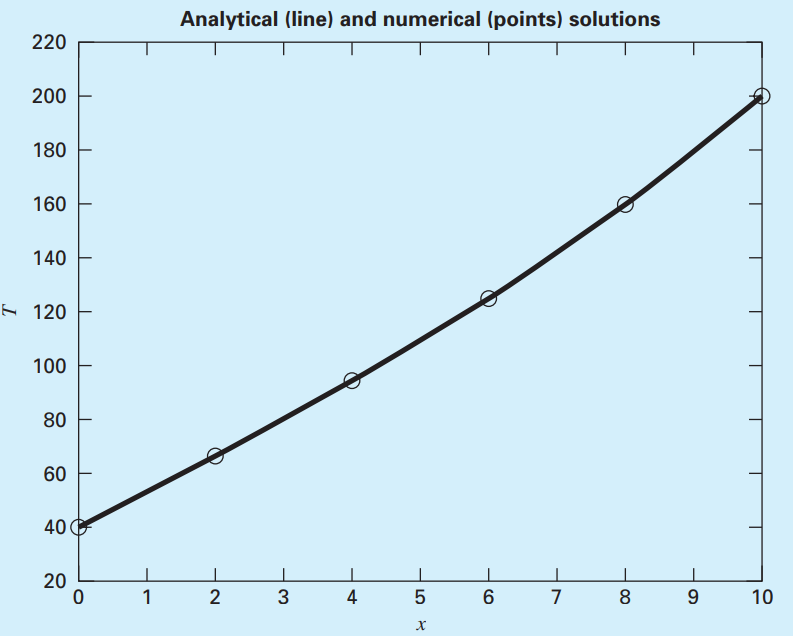
\includegraphics[width=1\linewidth]{fig_9_8}
	\caption{\textsf{A plot of temperature versus distance along a heated rod. Both analytical (line) and numerical (points) solutions are displayed.}}
	\label{fig:fig_9_8}
\end{figure}

In addition to being a linear system, notice that Eq. (9.28) is also tridiagonal. We can use an efficient solution scheme like the M-file in Fig. 9.6 to obtain the solution:
\begin{lstlisting}[numbers=none]
>> e=[0 -1 -1 -1];
>> f=[2.04 2.04 2.04 2.04];
>> g=[-1 -1 -1 0];
>> r=[40.8 0.8 0.8 200.8];
>> Tridiag(e,f,g,r)
ans = 65.9698 93.7785 124.5382 159.4795
\end{lstlisting}
The system is tridiagonal because each node depends only on its adjacent nodes.
Because we numbered the nodes sequentially, the resulting equations are tridiagonal. Such
cases often occur when solving differential equations based on conservation laws.


\pagebreak
\subsection*{PROBLEMS}

\begin{multicols}{2}
\begin{enumerate}
	\item Determine the number of total flops as a function of the number of equations $n$ for the tridiagonal algorithm (Fig. 9.6).
	\item Use the graphical method to solve
		$$2x_{1}-6x_{2}=-18$$
		$$-x_{1}+8x_{2}=40$$
		Check your results by substituting them back into the equations.
	\item Given the system of equations
		$$0.77x_{1}+x_{2}=14.25$$
		$$1.2x_{1}+1.7x_{2}=20$$
		\begin{enumerate}
			\item Solve graphically and check your results by substituting them back into the equations.
			\item On the basis of the graphical solution, what do you expect regarding the condition of the system?
			\item Compute the determinant.
		\end{enumerate}
	\item Given the system of equations
		$$2x_{2}+5x_{3}=1$$
		$$2x_{1}+x_{2}+x_{3}=1$$
		$$3x_{1}+x_{2}=2$$
		\begin{enumerate}
			\item Compute the determinant.
			\item Use Cramer’s rule to solve for the x’s.
			\item Use Gauss elimination with partial pivoting to solve for the x’s. As part of the computation, calculate the determinant in order to verify the value computed in (a)
			\item Substitute your results back into the original equations to check your solution.
		\end{enumerate}
	\item Given the equations
		$$0.5x_{1}-x_{2}=-9.5$$
		$$1.02x_{1}-2x_{2}=-18.8$$
		\begin{enumerate}
			\item Solve graphically.
			\item Compute the determinant.
			\item On the basis of \textbf{(a)} and \textbf{(b)}, what would you expect regarding the system’s condition?
			\item Solve by the elimination of unknowns.
			\item Solve again, but with $a_{11}$ modified slightly to 0.52. Interpret your results.
		\end{enumerate}
	\item Given the equations
		$$10x_{1}+2x_{2}-x_{3}=27$$
		$$-3x_{1}-5x_{2}+2x_{3}=-61.5$$
		$$x_{1}+x_{2}+6x_{3}=-21.5$$
		\begin{enumerate}
			\item Solve by naive Gauss elimination. Show all steps of the computation.
			\item Substitute your results into the original equations to check your answers.
		\end{enumerate}
	\item Given the equations
		$$2x_{1}-6x_{2}-x_{3}=-38$$
		$$-3x_{1}-x_{2}+7x_{3}=-34$$
		$$-8x_{1}+x_{2}-2x_{3}=-20$$
		\begin{enumerate}
			\item Solve by Gauss elimination with partial pivoting. As part of the computation, use the diagonal elements to calculate the determinant. Show all steps of the computation.
			\item Substitute your results into the original equations to check your answers.
		\end{enumerate}
	\item Perform the same calculations as in Example 9.5, but for the tridiagonal system:
\begin{equation}
\left [\begin{array}{ccccc}
0.8 	& -0.4 	& 	 	\\
-0.4	& 0.8	& -0.4 	\\
 		& -0.4 	& 0.8	\\
\end{array} \right ]
\begin{Bmatrix}
x_{1}\\
x_{2}\\
x_{3}\\
\end{Bmatrix} =
\begin{Bmatrix}
41\\
25\\
105\\
\end{Bmatrix}
\end{equation}
	\item Figure P9.9 shows three reactors linked by pipes. As indicated, the rate of transfer of chemicals through each pipe is equal to a flow rate ($Q$, with units of cubic meters per second) multiplied by the concentration of the reactor from which the flow originates ($c$, with units of milligrams per cubic meter). If the system is at a steady state, the transfer into each reactor will balance the transfer out. Develop mass-balance equations for the reactors and solve the three simultaneous linear algebraic equations for their concentrations.
	\item A civil engineer involved in construction requires 4800, 5800, and 5700 $m^{3}$ of sand, fine gravel, and coarse gravel, respectively, for a building project. There are three
	\begin{figure}[H]
		\centering
		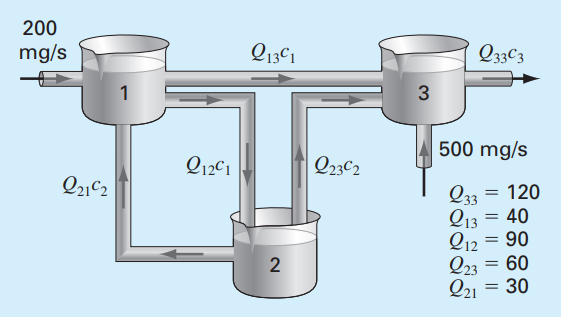
\includegraphics[width=1\linewidth]{fig_9_9}
		\caption{\textsf{Three reactors linked by pipes. The rate of mass transfer through each pipe is equal to the product of flow \textbf{$Q$} and concentration $c$ of the reactor from which the flow originates.}}
		\label{fig:fig_9_9}
	\end{figure}
	pits from which these materials can be obtained. The composition of these pits is
	\begin{figure}[H]
		\centering
		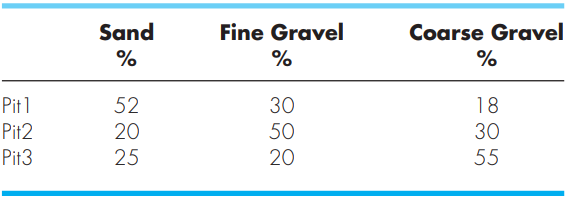
\includegraphics[width=1\linewidth]{fig_9_10}
	\end{figure}
	How many cubic meters must be hauled from each pit in order to meet the engineer’s needs?
	\item An electrical engineer supervises the production of three types of electrical components. Three kinds of material - metal, plastic, and rubber—are required for production. The amounts needed to produce each component are
	\begin{figure}[H]
		\centering
		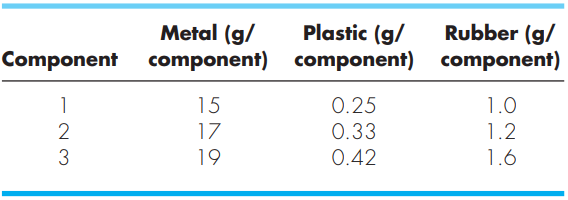
\includegraphics[width=1\linewidth]{fig_9_11}
	\end{figure}
	If totals of 2.12, 0.0434, and 0.164 kg of metal, plastic, and rubber, respectively, are available each day, how many components can be produced per day?
	\item As described in Sec. 9.4, linear algebraic equations can arise in the solution of differential equations. For example, the following differential equation results from a steady-state mass balance for a chemical in a one-dimensional canal:
	$$0=D\frac{d^{2}c}{dx^{2}}-U\frac{dc}{dx}-kc$$
	where c = concentration, t = time, x = distance, D = diffusion coefficient, U = fluid velocity, and $k=a$ first-order decay rate. Convert this differential equation to an equivalent system of simultaneous algebraic equations. Given $D=2$, $U=1$, $k=0.2$, $c(0)=80$ and $c(10)=10$, solve these equations from $x=0$ to 10 and develop a plot of concentration versus distance.
	\item A stage extraction process is depicted in Fig. P9.13. In such systems, a stream containing a weight fraction $y_{in}$ of a chemical enters from the left at a mass flow rate of $F_{1}$. Simultaneously, a solvent carrying a weight fraction $x_{in}$ of the same chemical enters from the right at a flow rate of $F_{2}$. Thus, for stage $i$, a mass balance can be represented as
	$$ F_{1}y_{i-1}+F_{2}x_{i+1}=F_{1}y_{i}+F_{2}x_{i} $$
	\begin{flushright}
	(P9.13a)
	\end{flushright}
	At each stage, an equilibrium is assumed to be established between $y_{i}$ and $x_{i}$ as in
	$$ K=\frac{x_{i}}{y_{i}} $$
	\begin{flushright}
	(P9.13b)
	\end{flushright}
	where $K$ is called a distribution coefficient. Equation (P9.13b) can be solved for $x_{i}$ and substituted into Eq. (P9.13a) to yield
	$$y_{i-1}-(1+\frac{F_{2}}{F_{1}}K)y_{i}+(\frac{F_{2}}{F_{1}}K)y_{i+1}=0$$
	\begin{flushright}
	(P9.13c)
	\end{flushright}
	If $F_{1}=400 kg/h$, $y_{in}=0.1$, $F_{2}=800 kg/h$, $x_{in}=0$, and $K=5$, determine the values of $y_{out}$ and $x_{out}$ if a five-stage reactor is used. Note that Eq. (P9.13c) must be modified to account for the inflow weight fractions when applied to the first and last stages.
	\item A peristaltic pump delivers a unit flow ($Q_{1}$) of a highly viscous fluid. The network is depicted in Fig. P9.14. Every pipe section has the same length and diameter. The mass and mechanical energy balance can be simplified to obtain the
\end{enumerate}
\end{multicols}

\begin{figure}[H]
	\centering
	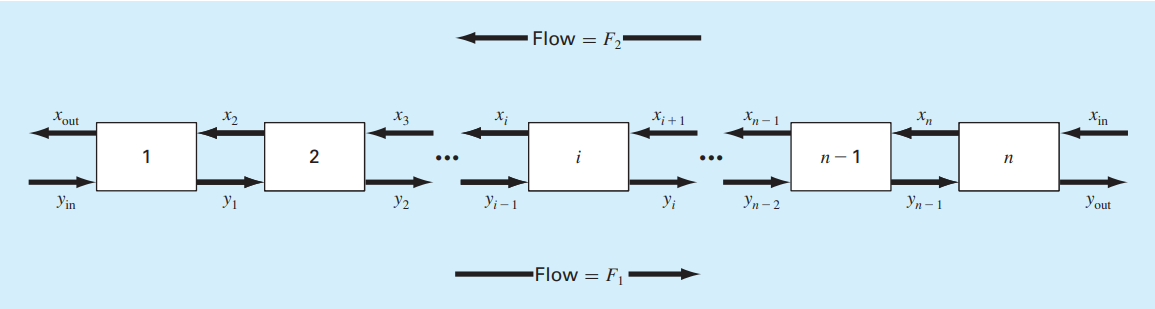
\includegraphics[width=1\linewidth]{fig_9_12}
	\caption{\textsf{A stage extraction process.}}
	\label{fig:fig_9_12}
\end{figure}
\pagebreak
\begin{multicols}{2}
	\begin{figure}[H]
		\centering
		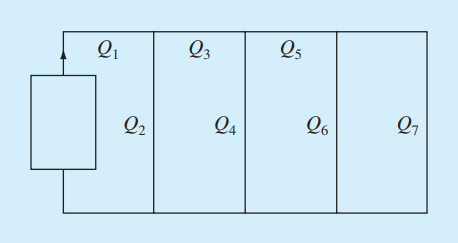
\includegraphics[width=1\linewidth]{fig_9_13}
		\caption{}
		\label{fig:fig_9_13}
	\end{figure}
	flows in every pipe. Solve the following system of equations to obtain the flow in every stream.

	$Q_{3}+2Q_{4}-2Q_{2}=0$ \hfill $Q_{1}=Q_{2}+Q_{3}$

	$Q_{5}+2Q_{6}-2Q_{4}=0$ \hfill $Q_{3}=Q_{4}+Q_{5}$

	$3Q_{7}-2Q_{6}=0$ \hfill $Q_{5}=Q_{6}+Q_{7}$
	\begin{enumerate}\setcounter{enumi}{14}
		\item A truss is loaded as shown in Fig. P9.15. Using the following set of equations, solve for the 10 unknowns, $AB$, $BC$, $AD$, $BD$, $CD$, $DE$, $CE$, $A_{x}$, $A_{y}$, and $E_{y}$.

	$A_{x}+AD=0$ \hfill $-24-CD-(4/5)CE=0$

	$A_{y}+AB=0$ \hfill $-AD+DE-(3/5)BD=0$

	$74+BC+(3/5)BD=0$ \hfill $CD+(4/5)BD=0$

	$-AB-(4/5)BD=0$ \hfill $-DE-(3/5)CE=0$

	$-BC+(3/5)CE=0$ \hfill $E_{y}+(4/5)CE=0$
		\begin{figure}[H]
			\centering
			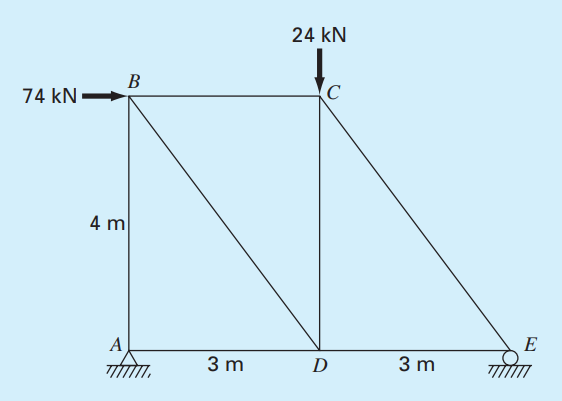
\includegraphics[width=1\linewidth]{fig_9_14}
			\caption{}
			\label{fig:fig_9_14}
		\end{figure}
		\item A \textit{pentadiagonal} system with a bandwidth of five can be expressed generally as
\[\begin{bmatrix}
f_{1} 	& g_{1}	& h_{1}	& 	 		& 	 		& 	 		& 		 	& 		\\
e_{2}	& f_{2} 	& g_{2}	& h_{2}	& 	 		& 	 		& 		 	& 		\\
d_{3} 	& e_{3}	& f_{3} 	& g_{3}	& h_{3}	& 	 		& 		 	& 		\\
	 	& 			& \cdot	& \cdot	& \cdot	& 	 		& 		 	& 		\\
	 	& 			& 	 		& \cdot	& \cdot 	& \cdot	& 		 	& 		\\
	 	& 			& 	 		&			& \cdot	& \cdot	& \cdot 	& 		\\
	 	& 			& 	 		&			& d_{n-1}	& e_{n-1}	& f_{n-1}	&g_{n-1}\\
	 	& 			& 	 		&			& 			& d_{n}	& e_{n} 	&f_{n}	\\
\end{bmatrix}\]

\[\times \begin{Bmatrix}
x_{1}\\
x_{2}\\
x_{3}\\
\cdot\\
\cdot\\
\cdot\\
x_{n-1}\\
x_{n}
\end{Bmatrix} = \begin{Bmatrix}
r_{1}\\
r_{2}\\
r_{3}\\
\cdot\\
\cdot\\
\cdot\\
r_{n-1}\\
r_{n}
\end{Bmatrix}\]
Develop an M-file to efficiently solve such systems without
pivoting in a similar fashion to the algorithm used for tridiagonal matrices in Sec. 9.4.1. Test it for the following case:
\[\begin{bmatrix}
8 	& -2	& -1	& 0		& 0		\\
-2	& 9 	& -4	& -1	& 0		\\
-1 	& -3	& 7 	& -1	& -2	\\
0 	& -4	& -2 	& 12	& -5	\\
0 	& 0		& -7 	& -3	& 15	\\
\end{bmatrix} \begin{Bmatrix}
x_{1}\\
x_{2}\\
x_{3}\\
x_{4}\\
x_{5}
\end{Bmatrix} = \begin{Bmatrix}
5\\
2\\
1\\
1\\
5
\end{Bmatrix}\]
	\item Develop an M-file function based on Fig. 9.5 to implement Gauss elimination with partial pivoting. Modify the function so that it computes and returns the determinant (with the correct sign), and detects whether the system is singular based on a near-zero determinant. For the latter, define "near-zero" as being when the absolute value of the determinant is below a tolerance. When this occurs, design the function so that an error message is displayed and the function terminates. Here is the functions first line:
	\begin{verbatim}
	function [x, D] = GaussPivotNew(A, b, tol)
	\end{verbatim}
	where $D =$ the determinant and $tol =$ the tolerance. Test your program for Prob. 9.5 with $tol = 1 \times 10^{-5}$.
	\end{enumerate}

\end{multicols}

\end{document}
